\documentclass{beamer}
\usepackage{lsfolien}
\usepackage[english]{babel}
\usepackage[utf8]{inputenc}

\myfootline{System Modelling and Semantic Web -- Spring 2021}{Hans-Gert Gräbe}

\newcommand{\ueberschrift}[1]{\begin{center}\bf #1\end{center}}

\title{Modelling Sustainable Systems\\ and Semantic Web\\[6pt]
  Development of Systems and Their Components
  \vskip1em}

\subtitle{Lecture in the Module 10-202-2309\\ for Master Computer Science}

\author{Prof. Dr. Hans-Gert Gräbe\\
\url{http://www.informatik.uni-leipzig.de/~graebe}}

\date{May 2021}
\begin{document}

{\setbeamertemplate{footline}{}
\begin{frame}
  \titlepage
\end{frame}}

\section{Open Systems}
\begin{frame}{Dissipative Systems and Steady States}

  The Theory of Dynamical Systems in the scope as discussed in this and the
  last lecture, describes \emph{internal dynamics} of systems.

  Our notion of a TS, however, assumes that components of a system in the
  execution dimension -- via their input/output (parametrised in the
  description form) -- are supplied with tasks and material by the system.

  Since our concept is recursive, this must be applied to \emph{all} systems,
  i.e.  they are always driven by a \emph{throughput of material and energy}.

  This is also stated by the TRIZ law of \emph{"energy conductivity" through
    all parts of the system}.
\end{frame}

\begin{frame}{Examples and Notions}
  Examples: Bénard cell, living beings, Earth's biosphere.  See
  \texttt{TDS.md}

  Notions (in the description form!): 
  \begin{itemize}
  \item eigentimes and eigenspaces
  \item limit cycles, attractors
  \item steady state and dissipative systems
  \end{itemize}
\end{frame}

\begin{frame}{Diagrams from (Holling 2001)}
  \begin{center}
    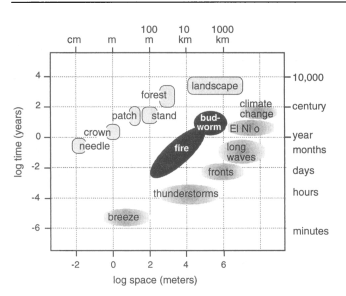
\includegraphics[width=.75\textwidth]{Holling-1.png}
  \end{center}
\end{frame}

\begin{frame}{Diagrams from (Holling 2001)}
  \begin{center}
    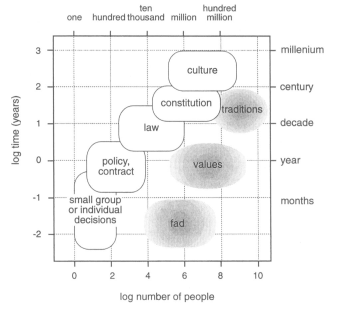
\includegraphics[width=.75\textwidth]{Holling-2.png}
  \end{center}
\end{frame}

\begin{frame}{Diagrams from (Holling 2001)}
  \begin{center}
    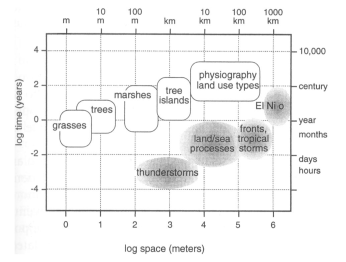
\includegraphics[width=.85\textwidth]{Holling-3.png}
  \end{center}
\end{frame}

\begin{frame}{Development of System and Components}

  \emph{Example:} A TS with two components -- the car body department of a car
  manufacturer with press subdepartment and coloring subdepartment.
    
  \begin{minipage}{.42\textwidth}\centering\vspace*{2em}
    \begin{tikzpicture}[line width=1pt]
        \node[draw,text width=3em, align=center] [circle] (A0) {CBD};
        \node[draw,below left=of A0, node distance=2em] [circle] (A1) {PS};
        \node[draw,below right=of A0, node distance=2em] [circle] (A2) {CS};
        \draw[-,dashed] (A0)--(A1) ;
        \draw[-,dashed] (A0)--(A2) ;
    \end{tikzpicture}\\[2em] Structural Organisation
  \end{minipage}\hfill
  \begin{minipage}{.55\textwidth}\centering
    \begin{tikzpicture}[line width=1pt,scale=.7,transform shape]
    \node[draw,text width=3em, align=center] [circle] (A0) {CBD};
    \node[draw,text width=2cm, align=center, above left=of A0] [rectangle] (I)
         {Input\\Metal Sheet}; 
    \node[draw,text width=2cm, align=center, above right=of A0] [rectangle] (O)
         {Output\\Finished Car Body}; 
    \node[draw,below left=of A0, node distance=2em] [circle] (A1) {PS};
    \node[draw,below right=of A0, node distance=2em] [circle] (A2) {CS};
    \draw[->] (I)--(A0) ;
    \draw[->] (A0)--(O) ;
    \draw[->] (A0) to[bend right] (A1) ;
    \draw[->] (A1) to[bend right] (A0) ;
    \draw[->] (A0) to[bend right] (A2) ;
    \draw[->] (A2) to[bend right] (A0) ;
    \end{tikzpicture}\\[2em] Workflow Organisation
  \end{minipage}
\end{frame}

\begin{frame}{Development of System and Components}

  \begin{minipage}{.4\textwidth}
    \emph{Continuation:} The press department is modernised, industrial robots
    are being used.  How does that affect the "neighbouring" systems?  What
    scenarios are conceivable?
  \end{minipage}\hfill
  \begin{minipage}{.55\textwidth}\centering
    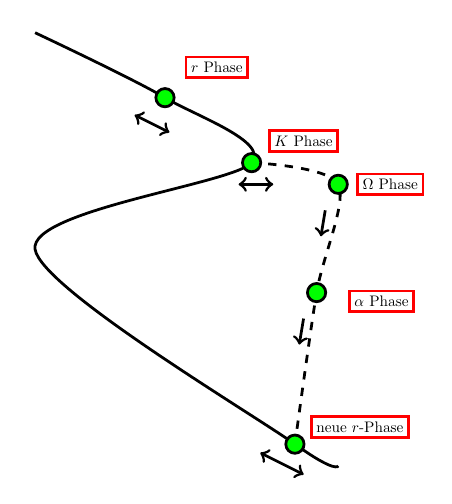
\begin{tikzpicture}[scale=.55,line width=1pt,transform shape]
      \node (A0) at (0,10) {};
    \node (A4) at (3,8.5) {};
    \node (A1) at (5,7) {};
    \node (A1a) at (7,6.5) {};
    \node (A2) at (0,5) {};
    \node (A3) at (7,0) {};
    \node (A5) at (6.5,4) {};
    \node (A6) at (6,.5) {};
    \draw plot [smooth] coordinates {(A0) (A4) (A1) (A2) (A6) (A3)};
    \node[draw=red] at (4.2,9.2) [rectangle] {$r$ Phase};
    \draw[<->] (2.3,8.1) -- (3.1,7.7) ;
    \node[draw=red] at (6.2,7.5) [rectangle] {$K$ Phase};
    \draw[<->] (4.7,6.5) -- (5.5,6.5) ;
    \node[draw=red] at (8.2,6.5) [rectangle] {$\Omega$ Phase};
    \draw[->] (6.7,5.9) -- (6.6,5.3) ;
    \node[draw=red] at (8,3.8) [rectangle] {$\alpha$ Phase};
    \draw[->] (6.2,3.4) -- (6.1,2.8) ;
    \draw[<->] (5.2,.3) -- (6.2,-.2) ;
    \draw[fill=green] (A4) circle (6pt) ;
    \draw[->,dashed] plot [smooth] coordinates {(A1) (A1a) (A5) (A6)};
    \draw[fill=green] (A1) circle (6pt) ;
    \draw[fill=green] (A1a) circle (6pt) ;
    \draw[fill=green] (A5) circle (6pt) ;
    \draw[fill=green] (A6) circle (6pt) ;
    \node[draw=red,fill=white] at (7.5,0.9) [rectangle] {neue $r$-Phase};
  \end{tikzpicture}
  \end{minipage}
\end{frame}
\begin{frame}{Diagrams from (Holling 2001)}
  \begin{center}
    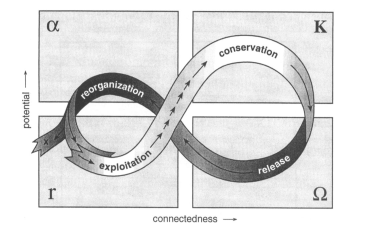
\includegraphics[width=.85\textwidth]{Holling-4.png}
  \end{center}
\end{frame}

\begin{frame}{Diagrams from (Holling 2001)}
  \begin{center}
    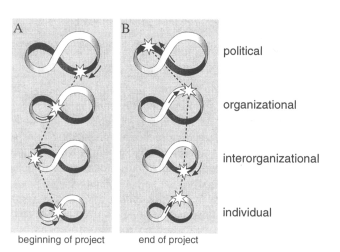
\includegraphics[width=.85\textwidth]{Holling-5.png}
  \end{center}
\end{frame}

\end{document}
